% !TeX spellcheck = sv_SE
\documentclass[a4paper]{article} 
\usepackage[T1]{fontenc} 
\usepackage[utf8]{inputenc} 
\usepackage[swedish]{babel}
\usepackage{graphicx}
\usepackage{multirow}
\usepackage{float}

\title{EDAA35\\ projekt} 
\author{Niklas Hedström \\dat15nhe@student.lu.se\and
	    Jakob Hök \\ dat15jh1@student.lu.se \and
	    Emil Wihlander\\ dat15ewi@student.lu.se} 
\date{2015--09--23} 

\begin{document}
\maketitle

\begin{abstract}
	I denna rapport undersöks exekveringstiden för tre olika sorteringsalgoritmer med samma värsta falls komplexitet vilket i detta fall är $O(n^2)$. Det används tre olika sorters indata med två olika storlekar, 500 tal och med 2000 tal där alla är heltal men det är olika sorterade från början. Den första är helst slumpgenerad, den andra är nästan helt sorterad och den sista är nästan omvänt sorterad. Alla algoritmerna körs 600 och ger ett medelvärde av de 600 gångerna ges och den processen görs 100 gånger för att sedan ta ut medelvärdet av de 100 medelvärdena. Sedan jämförs alla resultaten med varandra för att därefter vissa att \emph{Bubblesort} är den som presterar bäst på alla testerna.
\end{abstract}

\pagebreak

\section{Inledning}
Allt jämnt med att tekniken går framåt blir det viktigare för program att blir snabbare och då kan minsta nanosekund vara avgörande för om slutresultatet är bra eller dåligt. Ett sätt att få sitt program att jobba optimalt är att välja rätt sorts algoritm till rätt sorts arbete. Ett exempel kan vara att en sorteringsalgoritm kan vara bra på att sortera indata som är nästan helt sorterad men helt värdelös när det kommer till indata som är helt slumpgenererad, så det gäller att veta algoritmernas styrkor och svagheter när man väljer vilken algoritm man ska använda i programmet. Många gånger ska algoritmen köras flera tusen gånger och då kan valet av algoritm vara avgörande för slutresultatet, om en suboptimal algoritm körs en gång och gör en liten negativ differens i resultatet gör inte så stor skillnad men om den upprepas flera gånger blir den negativa differensen snabbt ett problem. Därför gäller det att man är noggrann när man väljer algoritm för att kunna spara viktiga nanosekunder i slutresultatet. 

\section{Bakgrund}
Syftet med dessa tester som vi har gjort är för att kunna jämföra hur \emph{Bubblesort}, \emph{Insertionsort} och \emph{Selectionsort} presterar i ett exekveringstidssammanhang för olika former av indata. Anledningen att valet föll på just dessa sorteringsalgoritmer då de har samma värsta falls komplexitet. Den hypotes som vi satte upp i början av laborationen var att \emph{Insertionsort} och \emph{Bubblesort} skulle vara likvärdiga i många tester men att \emph{Insertionsort} skulle vara oftare än inte vara snabbare än \emph{Bubblesort}, till sist skulle \emph{Selectionsort} vara den som tar längst tid varje gång då den har den värsta normal falls komplexiteten.\cite{sortingAlgoritm}

\section{Frågeställning}
\begin{itemize}
	\item I vilka fall av indata presterar respektive algoritm bäst?
	\item I vilka fall av indata presterar respektive algoritm sämst?
	\item Hur presterar algoritmerna i jämförelse med varandra för motsvarande indata?
\end{itemize}

\section{Metodik}
De program som användes för att utföra denna undersökning var \emph{Eclipse} där alla sorterings algoritmer skrevs i java. Sedan för att kunna köra algoritmerna flera gånger och få ut ett medelvärde så skrevs två program i R med hjälp av \emph{Rstudio}.  (förklaring av sorterings algoritmerna och hur det skrevs Emil). För att få fram indata som skulle sorteras användes först för den slumpgenererade listan ett eget skrivet program i java som hette randomSorted.java som använde javas \texttt{Random.nextInt()} för att kunna få trovärdigt slumpgenerade tal. Sedan för att få fram de andra två formerna av indata användes liknande program som hette almostNotSortedIndata.java och almostSortedIndata.java och de skapar indata-filer med ett visst antal element (i detta fall 2000 och 500). Den itererar då 500 eller 2000 gånger i en \texttt{for}-loop. I almostSortedIndata.java skapas för varje iteration "i" ett slumptal som kan vara ett värde från \texttt{i} till \texttt{i+3}. Alltså om vi är på iterationen 345 så kommer det slumpas ett tal mellan 345-348 och lägga in det i en fil. I almostNotSorted.java är det istället \texttt{i} till \texttt{i+3}.

När alla förberedelseuppgifter var klara blev undersökningens upplägg sådant att de tre olika algoritmerna vilket var \emph{Bubblesort}, \emph{Selectionsort} och \emph{Insertionsort} kördes 600 gånger och de gjordes på tre olika sorterade listor vilket var en slumpgenerade lista, en nästan helt sorterad lista och en nästan omvänt sorterad lista med två olika storlekar 500 och 2000 vilket i slutändan gjorde att det blev 18 olika mätningar. För varje gång en algoritm har körts 600 gånger så togs ett medelvärde av de körningarna och det gjordes 100 gånger för att kunna få ett medelvärde av medelvärdena. Att köra den 100 gånger gör att risken för outliers minskar vilket ger ett mer säkert resultat.

Efter varje körning skapades en plot av medelvärdena av medelvärdena och medelvärdet av dem räknades ut. I figur 1-3 ned kan man se exempel på plottar från mätningarna som gjordes med 500 element som var nästan sorterad från början.

\begin{figure}[H]
	\begin{center}
		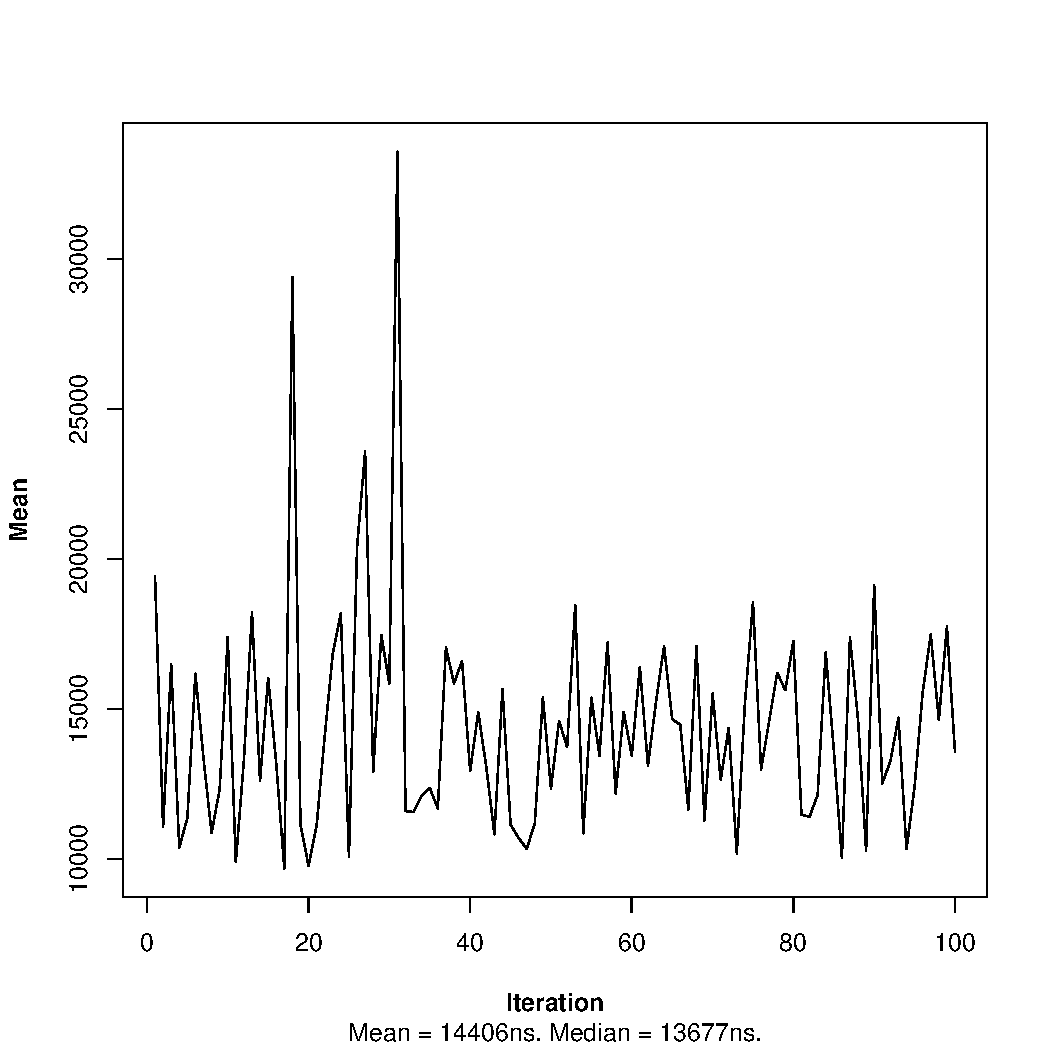
\includegraphics[scale=0.4]{output/500/AlmostSorted/insertionSort_almost_sorted_500_600_100.pdf}
		\caption{Plot för medelvärdena av medelvärdena som körts 600 gånger med sorteringsalgoritmen \emph{Insertionsort} på en lista med 500 element som var nästan helt sorterade.}
	\end{center}
\end{figure}

\begin{figure}[H]
	\begin{center}
		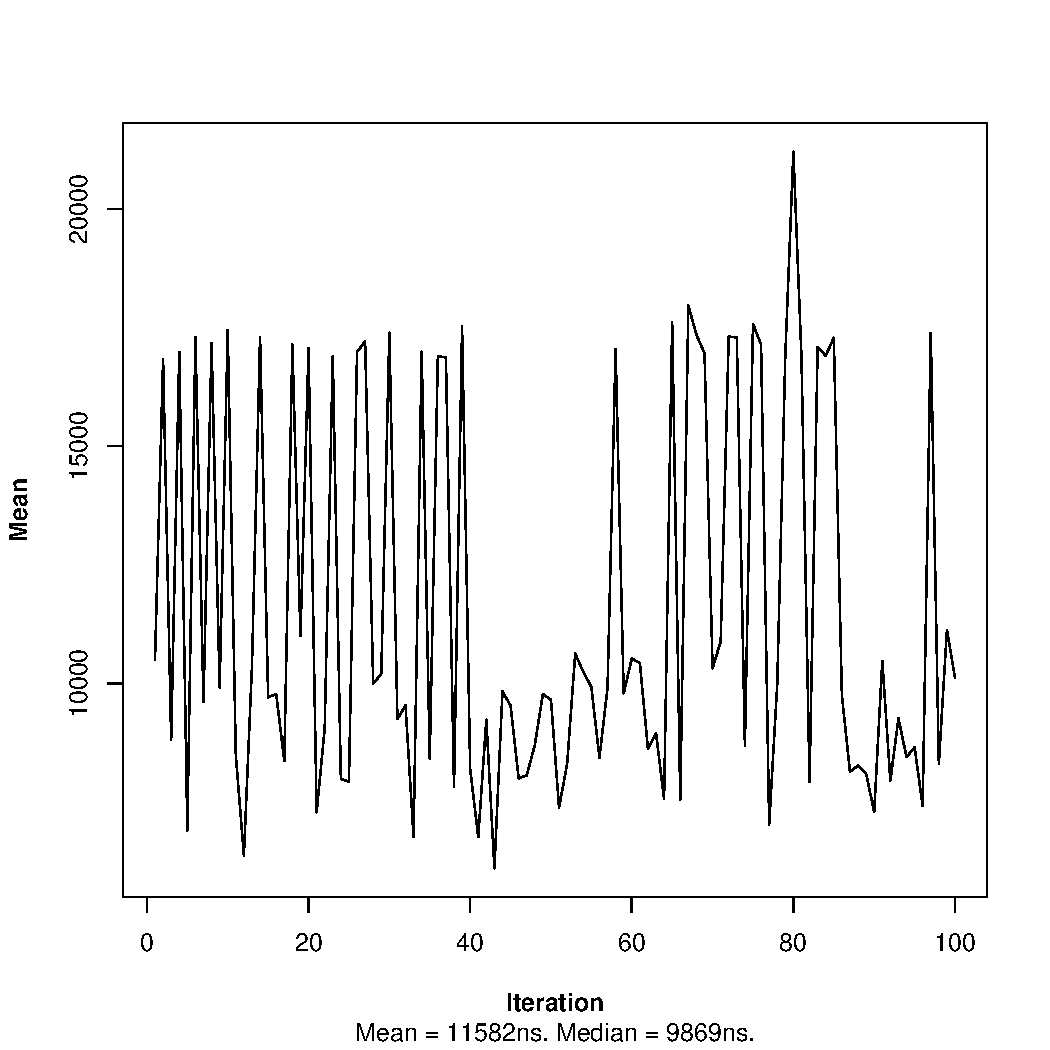
\includegraphics[scale=0.4]{output/500/AlmostSorted/bubbleSort_almost_sorted_500_600_100.pdf}
		\caption{Plot för medelvärdena av medelvärdena som körts 600 gånger med sorteringsalgoritmen Bubblesort på en lista med 500 element som var nästan helt sorterade.}
	\end{center}
\end{figure}

\begin{figure}[H]
	\begin{center}
		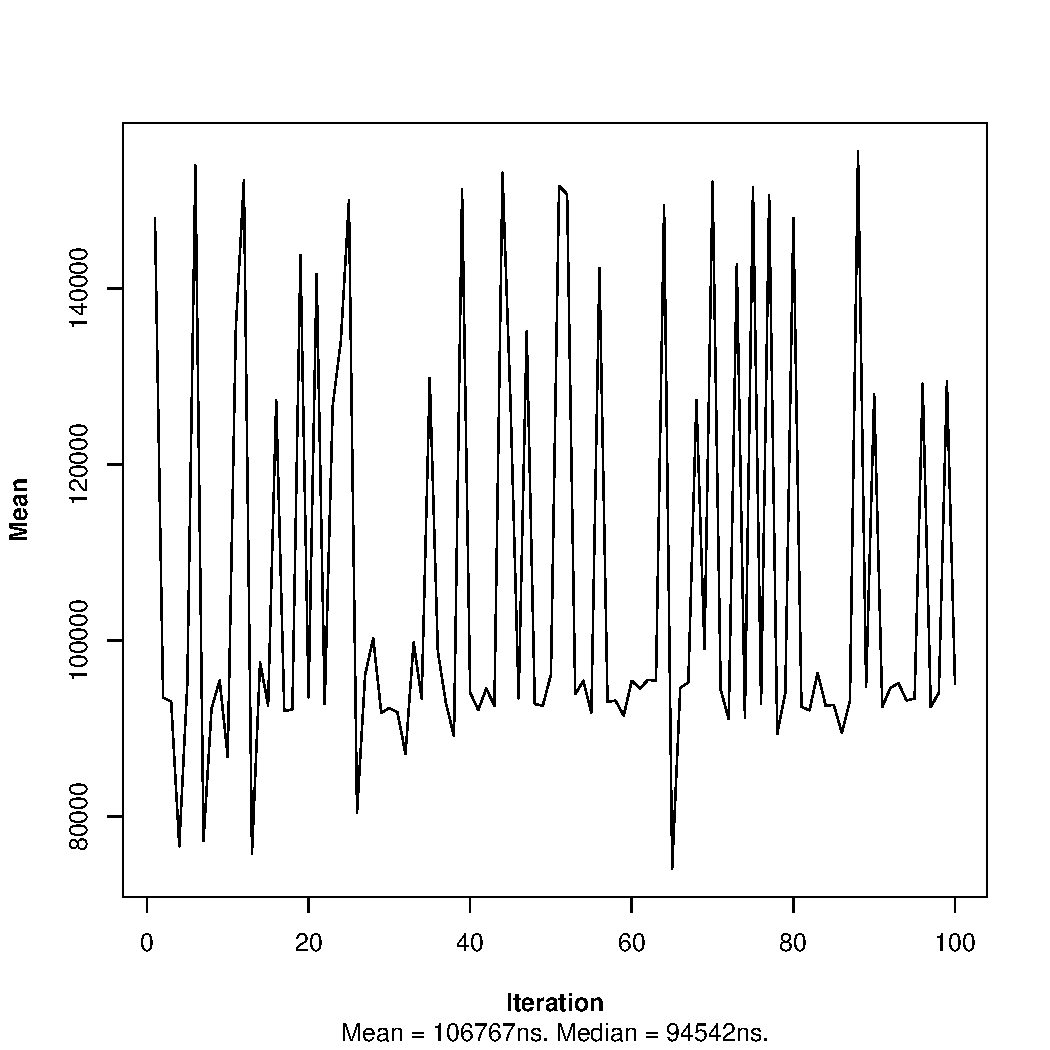
\includegraphics[scale=0.4]{output/500/AlmostSorted/selectionSort_almost_sorted_500_600_100.pdf}
		\caption{Plot för medelvärdena av medelvärdena som körts 600 gånger med sorteringsalgoritmen Selectionsort på en lista med 500 element som var nästan helt sorterade.}
	\end{center}
\end{figure}

\section{Resultat}
Här är en tabell över alla medelvärden och medianer som är framtagna från undersökningen med indata som hade 500 element i sig. 

Medelvärde: mv, Median: md 
\begin{table}[H]
	\begin{tabular}{r|c|c|c|}
		antal: 500 & Slumpgenererad & Nästan sorterad & Nästan omvänt sorterad \\ \hline
		\multirow{2}{*}{Bubblesort}    & mv: 3276ns & mv: 11582ns & mv: 4018ns \\
		                               & md: 2544ns & md: 9869ns & md: 2464ns \\ \hline
		\multirow{2}{*}{Selectionsort} & mv: 115834ns & mv: 106767ns & mv: 115260ns \\
		                               & md: 131243ns & md: 94542ns & md: 97796ns \\ \hline
		\multirow{2}{*}{Insertionsort} & mv: 9384ns & mv: 14406ns & mv: 6977ns \\
		                               & md: 7283ns & md: 13677ns & md: 5141ns \\ \hline	
	\end{tabular}
	\caption{Tabell med medelvärde och medianer för alla tester som gjordes med 500 element.}
\end{table}
\begin{table}[H]
	\begin{tabular}{r|c|c|c|}
		antal: 2000 & Slumpgenererad & Nästan sorterad & Nästan omvänt sorterad \\ \hline
		\multirow{2}{*}{Bubblesort}    & mv: 10177ns & mv: 19265ns & mv: 10992ns \\
		                               & md: 9304ns & md: 19320ns & md: 11017ns \\ \hline
		\multirow{2}{*}{Selectionsort} & mv: 1922456ns & mv: 1857603ns & mv: 1977647ns \\
		                               & md: 1910580ns & md: 1846435ns & md: 18918116ns \\ \hline
		\multirow{2}{*}{Insertionsort} & mv: 14040ns & mv: 27678ns & mv: 13828ns \\
		                               & md: 13581ns & md: 27089ns & md: 13492ns \\ \hline	
	\end{tabular}
	\caption{Tabell med medelvärde och medianer för alla tester som gjordes med 2000 element.}
\end{table}

\section{Diskussion}
Det man kan avgöra utifrån resultaten av mätningarna i vårt test är att \emph{Bubblesort} presterar bäst på alla olika former av indata vilket kan tyckas vara konstigt då de flesta andra källor som jämför sorteringsalgoritmer visar på att \emph{Insertionsort} skulle vara likvärdig eller bättre än \emph{Bubblesort} på de flesta formerna av indata.

Den sorteringsalgoritm som presterar svagast på alla testerna är \emph{Selectionsort} vilket inte är speciellt konstigt då \emph{Selectionsorts} värsta falls komplexitet är den samma som \emph{Selectionsorts} normal falls komplexitet. 

\section{Slutsats}
För att återkoppla till själva forskningsfrågorna kan man utifrån figur 4 och 5 se väldigt tydliga svar på frågorna. Den första frågan var ''I vilka fall av indata presterar respektive algoritm bäst?'' man kan tydligt se att \emph{Bubblesort} presterade bäst i alla tester som gjordes.

Den andra frågan var ''I vilka fall av indata presterar respektive algoritm sämst?'' det går även i denna fråga se att \emph{Selectionsort} presterade sämst i alla tester som utfördes.

Den sista frågan var ''Hur presterar algoritmerna i jämförelse med varandra för motsvarande indata?'' här kan man se att i alla olika former av indata är den förhållandevis skillnaden mellan algoritmerna omkring den samma.

\begin{thebibliography}{99}
	\bibitem{sortingAlgoritm} \emph{Sorting Algorithm Animations}, http://www.sorting-algorithms.com/, (2016 April 27, 11:30)
\end{thebibliography}

\end{document}